\begin{figure}[!htpb] 
\begin{center}
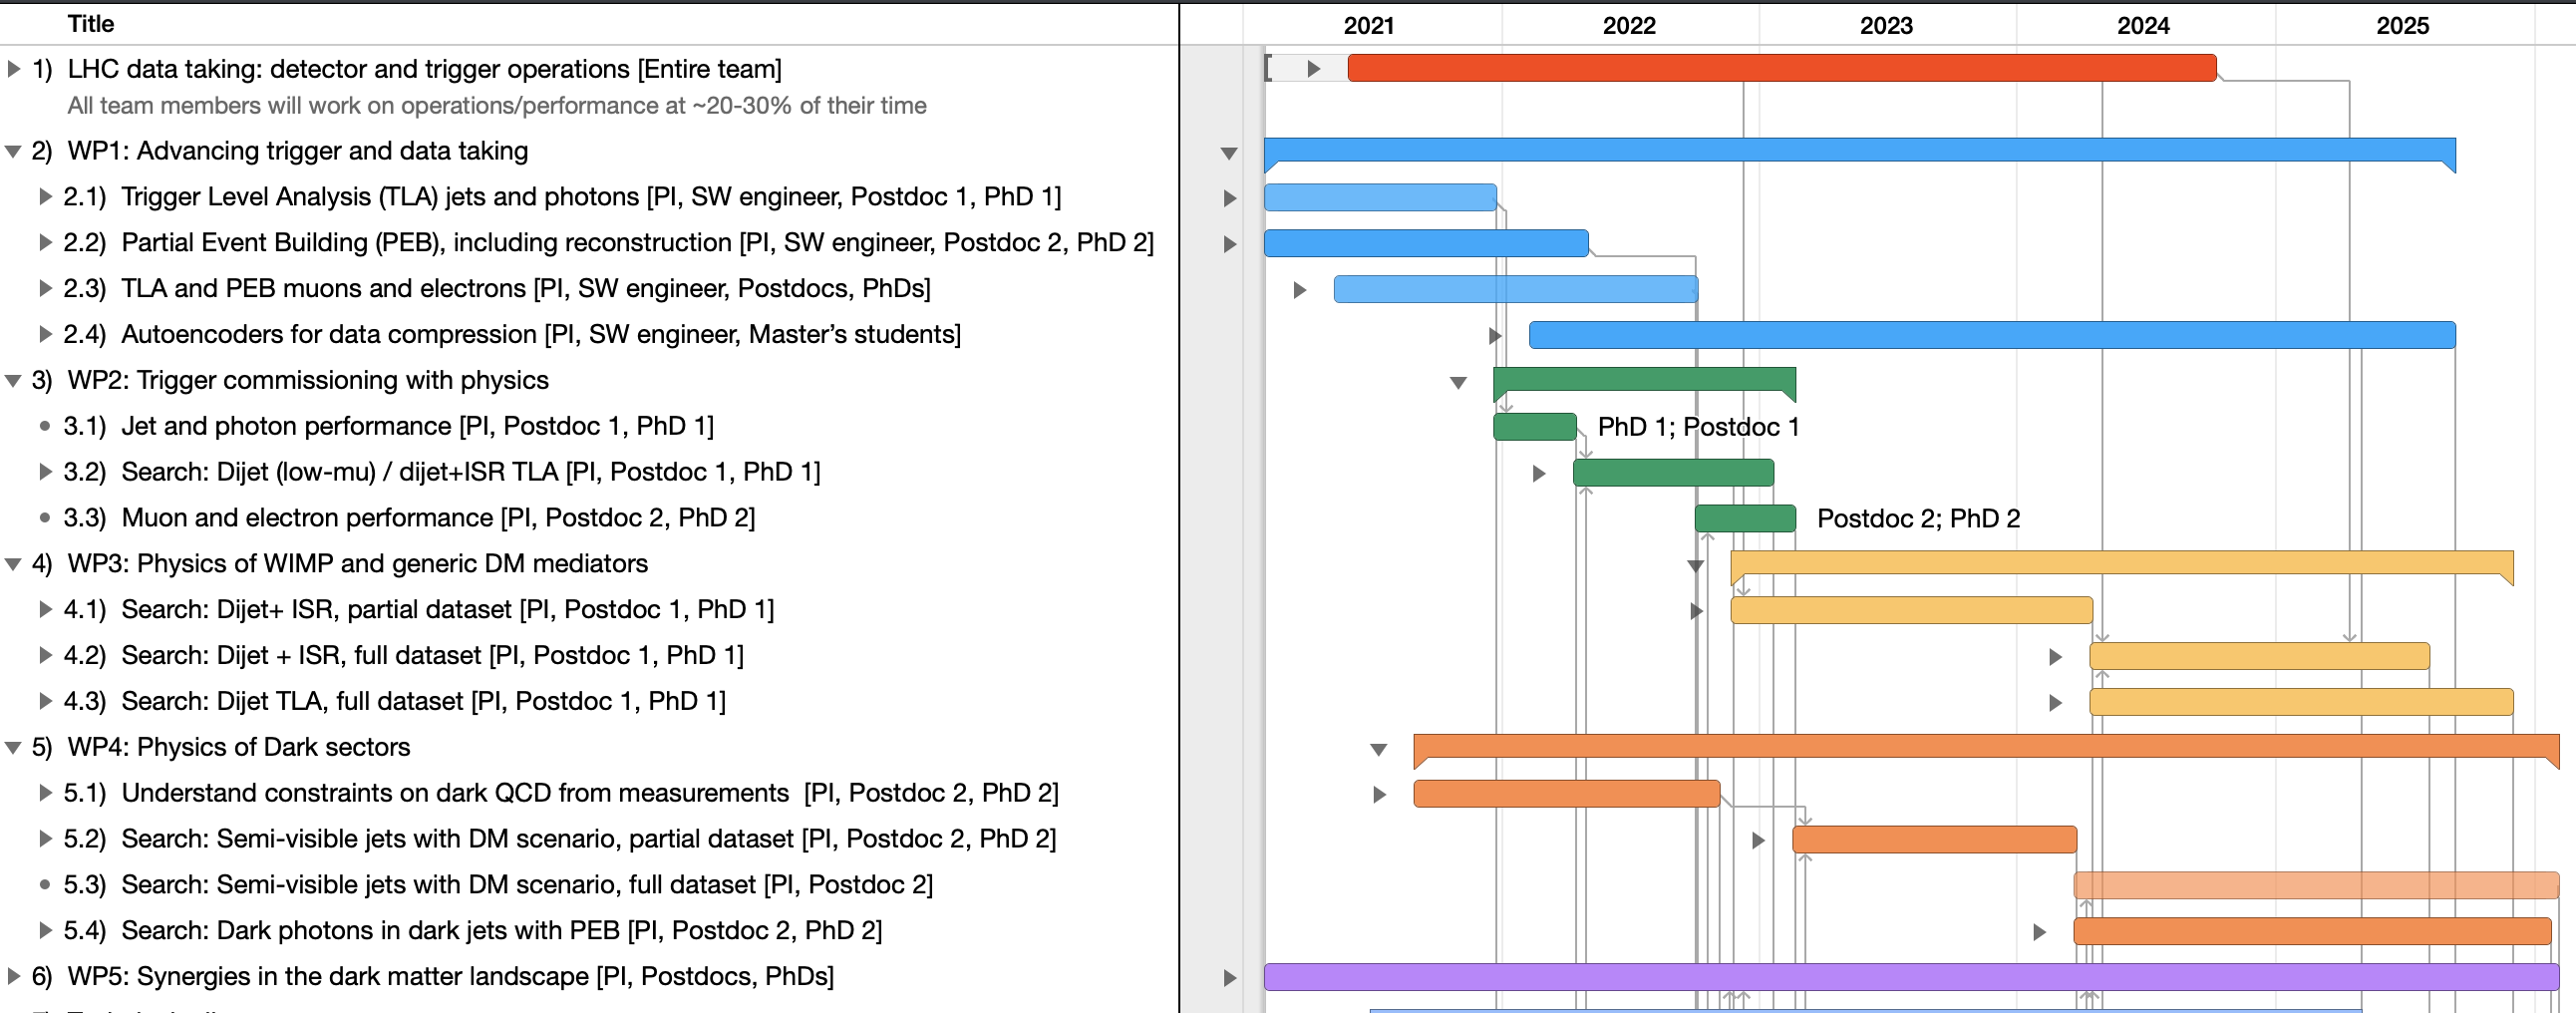
\includegraphics[width=\textwidth]{figs_B2/gantt}
\caption{\color{black}\label{fig:gantt} \small Sketch of project planning and division of work across team members.} 
\vskip2pt
\end{center}
\end{figure}
%\vskip5pt

The research team of \textsc{Realdark} that I will lead as a PI is composed by two postdoctoral researchers, two PhD students and one software engineer.
%Shift this to Resources
The postdoctoral researchers (PD1 and PD2) will be employed for the entirety of the project. 
The PhD students (PhD1 and PhD2) will work within \textsc{Realdark} for their 4-year thesis period. 
Each of the postdocs will work with one of the PhD students on the two physics objectives of WP3 and WP4 respectively, and related technical and commissioning tasks in WP1 and WP2. 
As PI, I will oversee all tasks in the project with day-to-day supervision and regular meetings, and have a hands-on involvement in more complex tasks as specified below. 
%allowing an effective sharing of supervision tasks. 
The software engineer will have a two-year contract at the beginning of the project to ensure the feasibility of the more software-intensive tasks in WP1. 
%end of shift to resources
Fig.~\ref{fig:gantt} provides a project planning schedule, including the breakdown of the work between the team members and intermediate milestones and deliverables marked with \textbf{[N]}. 
It has been prepared using the OmniPlan software~\cite{omni:plan},%Omniplan 
taking into account the interdependencies between the WPs and 
scheduling the work allocation in a way that ensures the feasibility of this ambitious project without overcommitting the team members. 

\subsection{WP1: Real-time analysis and data compression in ATLAS}

%The software implementation of TLA and TLA+PEB techniques and the calibration of physics objects recorded using these techniques represents a significant portion of the work in WP1. 
\textbf{TLA software implementation and calibration of trigger objects} As a preliminary input to this proposal, I have started working on a new Run-3 multithreaded HLT software algorithm that selects and writes out partially-built physics objects in the TLA stream. 
This algorithm will be more flexible than its Run-2 counterpart, and can handle any physics objects. 
By the start of this proposal, we expect to obtain preliminary results of the use of this algorithm on TLA jets. 
In 2021, PI, PD1, PhD1 and the software engineer
will work on the readiness of the core software for photons and jets, on commissioning with cosmic data, and on their subsequent calibration \textbf{[1]}
The experience gained with photons will be used by P1 and PhD1 to implement and commission TLA electrons as well, while PD2 and PhD2 will focus on TLA muons \textbf{[3]}. 
%Initially, the TLA stream will contain both jets and photons to enable analyses in WP3 in a simple manner. 
As part of this work, we will contribute to the design and implementation of seed trigger chains and data streams that selectively record one or more TLA objects simultaneously, optimizing according to the use cases in WP3 and WP4. 
The finalized TLA software streams will be ready in Q3 2022, allowing sufficient time for validation with data prior to the LHC production period. \\
\textbf{PEB software implementation and reconstruction} In Q1-Q2 2021, Prior to the implementation of TLA muons, PD2 and PhD2 will deploy the core software to write out user-defined regions of the detector together with TLA objects, 
%based on the Run-2 example for muons~\cite{ToBeCited}  and 
taking into account the optimization between CPU and storage costs mentioned in Sec.~\ref{subsub:TriggerRecoSoftware}~\textbf{[2]}. 
%strike a balance between the use of computing-expensive HLT algorithms to be able to drop raw detector data, and delaying running those algorithms until later at the cost of a larger event size. 
%The Cost Monitoring framework and test events storing different levels of detector information, informed by the calibration and reconstruction work as well as by the sensitivity studies, will be evaluated for this optimization. 
Subsequently, they will test the TLA+PEB implementation on early data and work together with the software engineer on the implementation of dedicated reconstruction algorithms for partial detector input, taking advantage of the experience gained with TLA electrons and muons~\textbf{[3]}. 
At the end of this work, expected for Q3 2022, we will publish a technical paper describing the combined TLA and PEB implementation within the ATLAS trigger (Q4 2022) \textbf{[5]}. \\
\textbf{Identification and calibration of TLA jets, photons, electrons and muons} Throughout 2021 and 2022, PhDs and postdocs will contribute to the algorithms for the identification and calibration of the HLT physics objects that they have implemented in TLA and PEB. 
In this proposal, we will focus on new HLT pile-up suppression techniques using calorimeter information against techniques using tracking information. 
The performance of this calibration will be studied in WP2 and documented in the technical papers in \textbf{[3]} and \textbf{[7]}.\\
Together with the performance studies, this work will be part of the students' ATLAS authorship qualification task.
\textbf{Data compression with autoencoders} Throughout the course of this proposal, the software engineer and I will supervise Master's students that study the performance, implementation and characteristics of autoencoder networks used to compress ATLAS data. 
The outcome of this work will be a test implementation in system that emulates a HLT computing node, preparing the ground for an implementation in the HL-LHC trigger and computing system~\textbf{[7]}. 
This work will be documented in technical publications, detailing preliminary and final work \textbf{[8,11]}.

\subsection{WP2: Commissioning the upgraded ATLAS trigger with physics}

\textbf{HLT object performance} Over the course of the early LHC data taking (2021-2022), 
PD1 and PhD1 will determine the performance of HLT jets and photons with early data, while PD2 and PhD2 will focus on the performance of HLT and PEB electrons and muons. \\
\textbf{Searches and measurements of the dijet mass spectrum} After the trigger jet and photon performance is well understood, PD1 and PhD1 and I will measure the dijet mass spectrum using a limited amount of data. 
We will select inclusive dijet events, and events where dijets are produced in association with a photon
%, first using offline jets and TLA jets, and then using TLA+PEB jets, for comparison with simulation and Run-2 data. 
This will lead to a prototype of the dijet and dijet+ISR TLA searches within the RECAST framework~\textbf{[9]}.   
PD2 and PhD2 will repeat this exercise with electrons and muons in a measurement of the $Z$ and $J/\psi$ peaks, 
to be included with the jet and photon performance work in a dedicated technical publication~\textbf{[10]}. 
If the LHC provides a dataset that surpasses the Run-2 sensitivity for either dijet and dijet+ISR searches, 
PD1, PhD1 and I will work with ATLAS collaborators towards publication of the result of these searches in Q2 2023~\textbf{[11]}.

\subsection{WP3: Dark matter mediator searches}

WIMP mediator searches and the interpretation of their results will be the main physics focus of PD1 and PhD1.\\ \indent
\textbf{Dijet+ISR TLA search} This search relies on calibrations and data analysis code developed and tested in WP1 and WP2.
%PD1 and PhD1 will perform the sensitivity and literature studies to deploy trigger chains seeding these TLAs prior to 2022, 
PD1 and PhD1 will refine the WP1 jet calibration for a high-statistics search (e.g. for pile-up suppression suppression techniques for the low-$p_{\mathrm{T}}$ resonance jets) and repeat the performance studies from WP2 with a larger dataset. 
PD1 and PhD1 will take advantage of WP2 RECAST implementation of the dijet+ISR mass spectrum to estimate backgrounds and produce inputs to run the statistical analysis.
PD1 and PhD1 will collaborate with colleagues from OSU, Oregon and Heidelberg on two publications, one using the first part of the dataset where the Run-2 sensitivity is surpassed~\textbf{[12]} in 2024, and one using the full Run-2 dataset~\textbf{[13]} in Q2 2025.\\ 
\textbf{Dijet TLA search} PD1 and I will remain involved in the full ATLAS Run-3 TLA with an advisory role. 
We will provide the WP2 RECAST implementation, and combine Run-2 and Run-3 results for a legacy TLA publication covering both LHC runs in Q3 2025 \textbf{[14]}. 
Dijet searches are sensitive to a variety of new physics signals (see Sec.~\ref{sub:stateOfTheArtTheory}): code and results from WP3 searches will be input to WP5 for broad dissemination. 

\subsection{WP4: Dark QCD searches}

Dark QCD searches and the interpretation of their results will be the main physics focus of PD2 and PhD2. 
Both searches in WP4 will require preliminary work and collaborations to decide on the optimal parameter space to target, described in WP5 below. 
This will be done within the first and second year of this proposal and culminate in a public document (ATLAS PUB note) on the reinterpretation of measurements and existing searches for a variety of dark QCD benchmark models in Q3 2022. 
This will inform the configuration for the TLA+PEB stream to be implemented upon the LHC restart in Q1-Q2 2023, 
together with the preliminary studies on the suppression of QCD background to implement at the HLT. \\
\textbf{Semi-visible jet search} This search will be the first to be tackled.
% as it relies on studies and analysis code in WP1-3 given the relative similarity of the two signatures. 
PD2 and PhD2 will bring their expertise to search for low-mass particles decaying into semi-visible jets in TLA+PEB, and work with colleagues from the University of Witswatersrand who will focus on the high-mass region with traditional techniques. 
This continues an existing collaboration started within my StG, which we expect to be supported by the ERC "Implementing Agreements" program during 2020.
We will publish this search with an intermediate dataset in Q2 2024~\textbf{[15]}, and continue our involvement in the full-dataset search with an advisory role. \\
\textbf{Composite jet search} This search shares many of the common PEB+TLA performance tools with the semi-visible jet search and proceeds in parallel during 2023. 
The bulk of the work will be done during 2024, first adapting WP1 and WP2 code and techniques for leptons within jets and then running the analysis chain, leading to a publication in Q4 2025~\textbf{[16]}. 
Throughout this period we will also work to make the TLA+PEB stream and the analysis tools available within ATLAS for other dark sector searches. 

\subsection{WP5: Interpretation, dissemination and synergies}

The work in WP5 is spread over all the timeline of this project and its hands-on components will involve the PI, the postdocs and the PhDs.
A \textbf{two-weeks workshop} with other non-LHC communities, involving experts and authors of the theory benchmarks for searches in this proposal who agreed to participate~\cite{ToBeCited} %Felix & co
will be organized in Q3 2021 within the iDMEu initiative. 
The workshop will be hosted at Lund for the first week and at CERN for the second week (with videoconference available in both), to discuss the state-of-the-art of dark QCD theory and experiment and understand current constraints including dark meson searches, non-collider and astrophysical constraints. \\
Together with each technical and physics publication we will share our results on HEPData and on plots that summarize searches from different techniques and experiments constraining the same model. Within iDMEu, we will also extend the benchmarks for these plots to dark QCD models, with a first iteration expected after the Lund/CERN workshop. \\
We will also make common-interest software in WP1 (e.g. compression, non-standard object reconstruction) and WP2-4 (RECAST analyses in REANA) available in the ESCAPE Software Catalogue as part of the DM Virtual Environment, and on the HSF webpages. 
This will include documentation and working examples for enhancing the usability and impact of the shared software. \\
Finally, I will write a review of the state of the art of LHC searches at colliders at the end of this project~\textbf{[17]}. 

%\textbf{Defining search targets} 
%Through workshops and discussions with the theory community, PD2 
%\textbf{Performance studies} During Q, the performance studies in WP2 will be extended to muons and electrons in busier hadronic environments, with a focus on the identification of variables and analysis techniques that can be used to minimize the impact of pile-up and reduce SM backgrounds already at the trigger level. 



